\chapter{Algorithms and Approaches for Terrain LOD}
\section{Basics of Terrain LOD}
\subsection{Terrain Data Representation}
One way of representing terrains is using \textit{heightmaps}.
A heightmap is a $n\times n$-grid that contains 
the height value $y$ for each $(x,z)$-position.
Positions are always spaced evenly in a grid-like manner,
but the distance between two neighboring vertices is variable
and can be set by the terrain programmer.

The main advantage of heightmaps is that it allows for very simple storage and manipulation of height data.
Terrain height data can easily be stored as grayscale images,
where low grayscale values represent low areas of terrain and vice versa for
high grayscale values. Looking up a height value for a given $(x,z)$-position is easy as well,
which consists of a simple lookup at the given position.
Figure 1 shows a $2000 \times 2000$ heightmap of the mountain Dom in Valais, Switzerland.
\begin{figure}
  \centering
  
\includegraphics[width=0.44\textwidth]{dom}
  \caption{$2000 \times 2000$ heightmap of the mountain Dom in Valais, Switzerland retrieved from SwissTopo \cite{alti3d}.}
\end{figure}

An alternative to the heightmap is the \textit{triangulated irregular network (TIN)} data structure.
A TIN consists of a collection of 3D vertices, where 
the arrangement of vertices can be irregular. Figure 2 shows 
an example of a TIN.
\begin{figure}
  \centering
  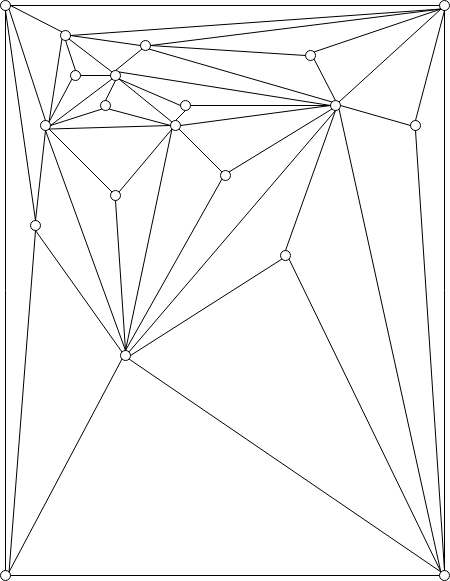
\includegraphics[width=0.52\textwidth]{tin-example}
  \caption{Example of a TIN. Note that the upper area represents a terrain area with many changes 
  (e.g. mountains, hills, etc.), and the lower area represents areas with few changes (e.g. flat areas)}.
\end{figure}


The main advantage of TINs is that fewer polygons need to be used for 
e.g. smooth terrain areas. Another advantage is that
special terrain features can be modelled 
which are usually difficult to model with heightmaps, such as overhangs, cliffs and caves, 
The disadvantage of TINs, however, is that the full $(x,y,z)$ coordinates need to be stored,
whereas with heightmaps, only the height value $y$ needs to be stored.

\subsection{Bintrees and Quadtrees}
Binary triangle trees (bintrees) and quadtrees are 
recursive data structures based on triangles and quads respectively.
Figure TODO shows a TODO.
The main advantage of bintrees and quadtrees is that 
LOD can be modelled very naturally with them.
Bintree/quadtree sections with few children correspond to a low level of detail and 
vice versa for bintree/quadtree sections with many children.

\subsection{Potential Problems During Terrain Rendering}
While terrain LOD algorithms dramatically improve the performance of terrain rendering, 
there are certain faults that can occur during rendering. 
\paragraph{T-junctions} T-junctions occur when 
\paragraph{Cracks} Cracks and holes in terrain occur when a higher LOD terrain section is bordered 
by a lower LOD terrain section. 

\section{ROAM}
ROAM (short for \textbf{R}eal-time \textbf{O}ptimally \textbf{A}dapting \textbf{M}eshes) 
is a terrain LOD algorithm developed by Duchaineau \textit{et al.} \cite{roam} published in 1997.
ROAM represents the terrain mesh using bintrees. The algorithm is mainly CPU-based, which 
can be attributed to the less developed state of GPU programming at the time.

The central idea of the algorithm is to use temporal coherence: the mesh from a previous frame $\mathbf{T}_{f-1}$ is used to compute 
the mesh of the current frame $\mathbf{T}$, rather than building up the mesh from ground up for each frame.
This is done using two priority queues: a split queue $\mathcal{Q}_s$ and a merge queue $\mathcal{Q}_m$.
The split queue contains splittable triangle pairs $()$
and the merge queue contains mergable triangle pairs $()$.
The elements of the priority queues are ordered by 
various geometric error metrics, which will be explained in the subsection ``Error Metrics''.
ROAM is a greedy algorithm, meaning it will always compute the most optimal mesh for each frame.

% [The algorithm is described in pseudocode below in algorithm 1.

% \newcommand{\pushcode}[1][1]{\hskip\dimexpr#1\algorithmicindent\relax}
% \begin{algorithm}
%   \caption{ROAM incremental greedy update}\label{alg:cap}
%   \begin{algorithmic}[1]
%   \Procedure{RoamIncrementalUpdate}{}
%   \If{$f = 0$} \Comment{Initial frame}
%     \State $\mathbf{T} \gets \text{base triangulation}$.
%     \State Clear $\mathcal{Q}_s, \mathcal{Q}_m$.
%     \State Compute priorities for triangles and diamonds $\in \mathbf{T}$ 
%     \State and insert them into $\mathcal{Q}_s$ and $\mathcal{Q}_m$.
%   \Else
%     \State $\mathbf{T} \gets \mathbf{T}_{f-1}$.
%     \State Update priorities for all elements $\in \mathcal{Q}_s$, $\mathcal{Q}_m$.
%   \EndIf
%   \While{\textbf{not} $\mathbf{T}$ is target size/accuracy \textbf{or} \\
%   \hskip\algorithmicindent maximum split priority $>$ minimum merge priority}
%     \If{$\mathbf{T}$ is too large or accurate}
%       \State Find lowest priority $(T, T_B) \in \mathcal{Q}_m$. 
%       \State Merge $(T, T_B)$.
%       \State Remove all merged children from $\mathcal{Q}_s$.
%       \State Add merge parents $T, T_B$ to $\mathcal{Q}_s$.
%       \State Add all newly mergable diamonds to $\mathcal{Q}_m$.
%     \Else \Comment{$\mathbf{T}$ is too small or inaccurate}
%       \State Find highest priority $T \in \mathcal{Q}_s$.
%       \State Force-split $T$.
%       \State Remove $T$ and other split triangles from $\mathcal{Q}_s$.
%       \State Add any new triangles $\in \mathbf{T}$ to $Q_s$.
%       \State Remove from $Q_m$ any diamonds whose children were split.
%       \State Add all newly mergable diamonds to $\mathcal{Q}_m$.
%     \EndIf
%   \EndWhile
%  \EndProcedure
%   \end{algorithmic}
% \end{algorithm}]

\subsection{Error Metrics}
The error metrics used for the priority queues are the following:

\paragraph{Wedgies} The so-called \textit{Wedgies} are nested bounding volumes around triangles that are computed 
while building an initial mesh at the beginning of the algorithm.
A wedgie is defined to contain the entire $x$ and $y$ extent % TODO is this the right coordinate system? 
of a triangle and the height $z$ including some additional space above and below the highest and lowest points,
respectively.

\paragraph{Geometric Screen Distortion}

\paragraph{Other Metrics} Other priority metrics mentioned include 

\subsection{Reported Performance and Conclusion}
Duchaineau et al. report that the runtime of ROAM is proportionate to the 
number of triangle changes.

\section{Röttger's Quadtree-based Algorithm}
TODO

\section{GeoMipMapping}
Geometrical Mipmapping (GeoMipMapping) is a terrain LOD approach developed by de Boer \cite{geomipmapping} in the year 2000.
Its reported main improvement over the previous algorithms is 

De Boer introduces the GeoMipMapping analogy based on texture mipmapping: multiple levels of 
GeoMipMaps get created for a terrain section, each for a level of detail, and depending on the distance
from the camera, the terrain section with the appropriate LOD level gets rendered.

\section{Geometry Clipmaps}
TODO

\section{CDLOD}
TODO

